
\section{Multivariate analysis}
\label{sec:mva}

After the traditional cut-based analysis presented in the previous section,
and combining the significance of the different event categories,
we end up with a $S/\sqrt{B}$ value of AAA.
%
Taking into account our more realistic simulation of the QCD background as
compared to previous studies, this is not too bad.
%
However, the attentive reader might have noticed that we have used
relatively 
loose kinematics cuts, for example in the Higgs mass window.
%
The motivation for this is that the $n$-tuples of signal and background
events, after our basic selection, are processed though a multivariate
analysis with the motivation to increase the signal over background
significance.


We now apply a basic MVA to the final output of the resolved and boosted analyses. The MVA used is a feed-forward artificial neural network with $N_{\mathrm{par}}\times5\times3\times1$ architecture, where $N_{\mathrm{par}}$ is the number of input parameters for the network. The MVA was trained for 50,000 GA generations with a cross-entropy error function. In Figure~\ref{fig:nnresponse} the neural network classification of events is demonstrated for both the resolved and boosted cases. In Figure~\ref{fig:exampleroc} the ROC curves for the two analyses are shown, demonstrating that the neural network is able to
perform well in both cases. Figure~\ref{fig:nnweights} shows the distribution of NN weights in both cases.


\begin{figure}[h]
\begin{center}
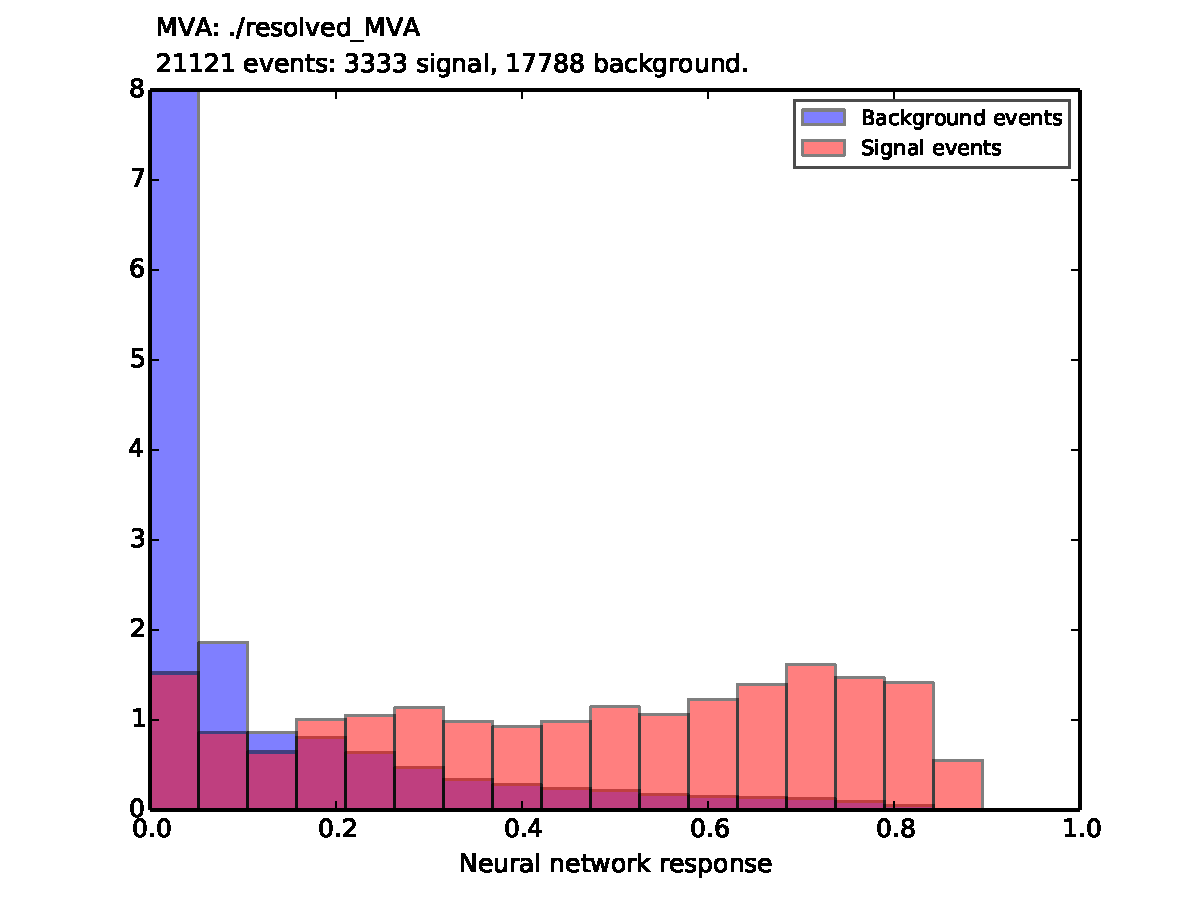
\includegraphics[width=0.49\textwidth]{plots/resolved_MVA_hist.pdf}
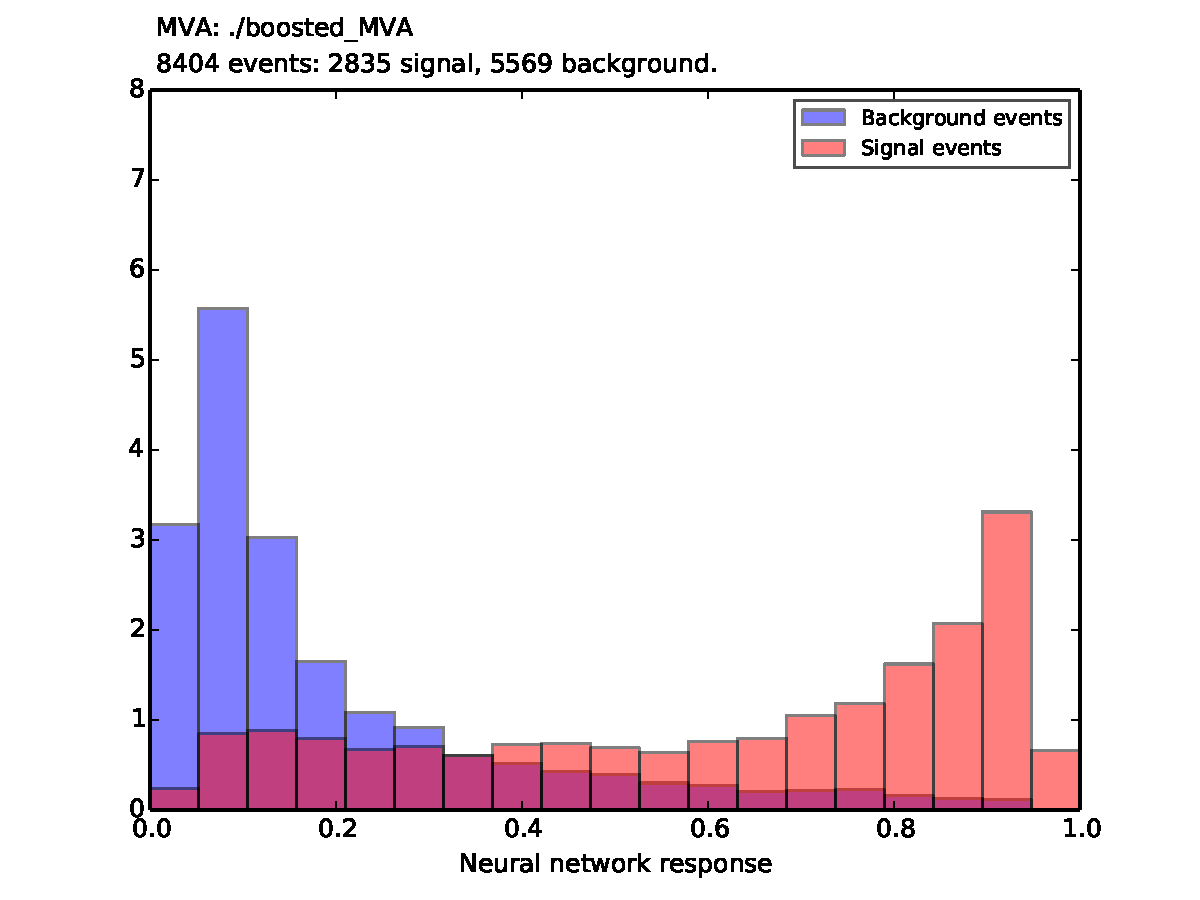
\includegraphics[width=0.49\textwidth]{plots/boosted_MVA_hist.pdf}
\caption{Neural network response demonstrated for the case of the resolved (left) and boosted (right) analyses. The frequency of background and signal events is plotted as a function of neural network output.}
\label{fig:nnresponse}
\end{center}
\end{figure}

\begin{figure}[h]
\begin{center}
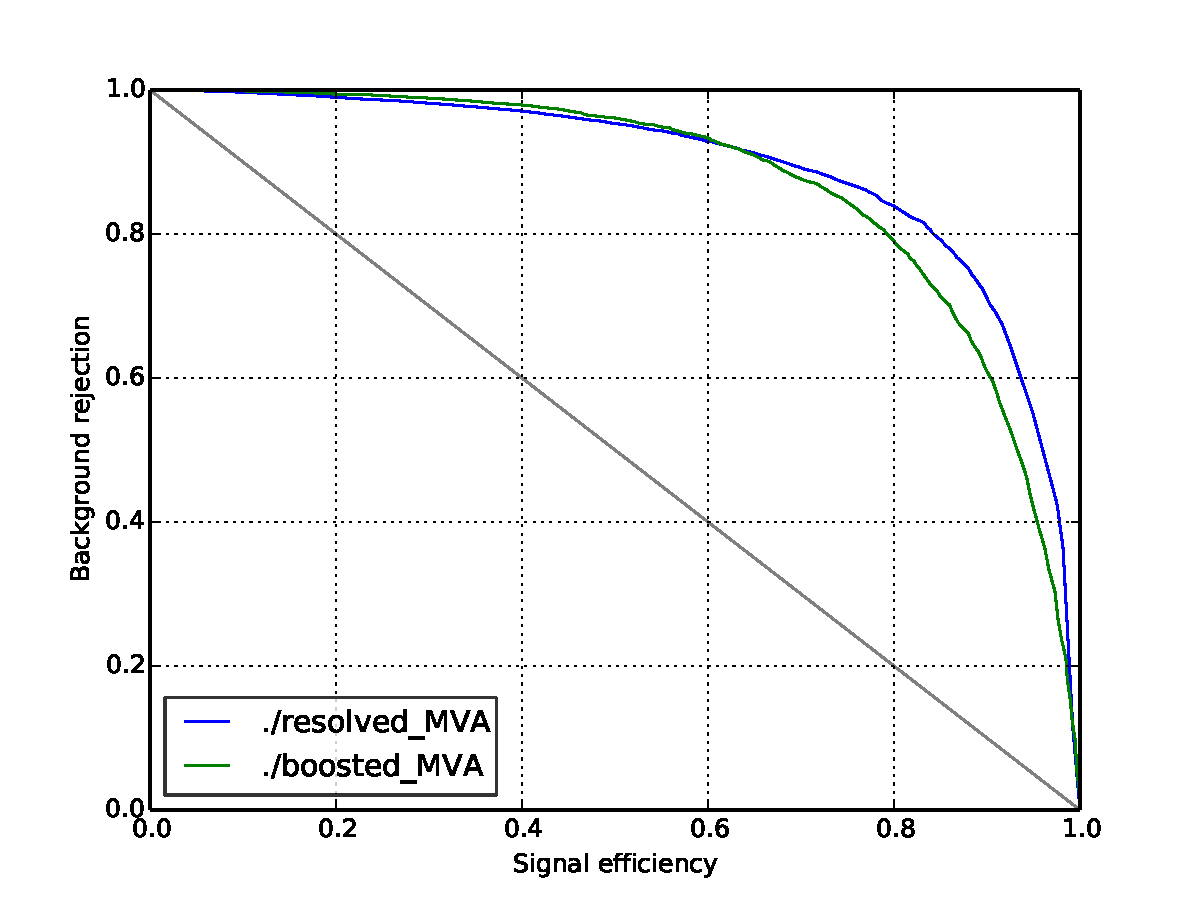
\includegraphics[width=0.95\textwidth]{plots/example_roc.pdf}
\caption{ROC curve for the neural network discriminant in the boosted (green) and resolved (blue) cases.}
\label{fig:exampleroc}
\end{center}
\end{figure}

\begin{figure}[h]
\begin{center}
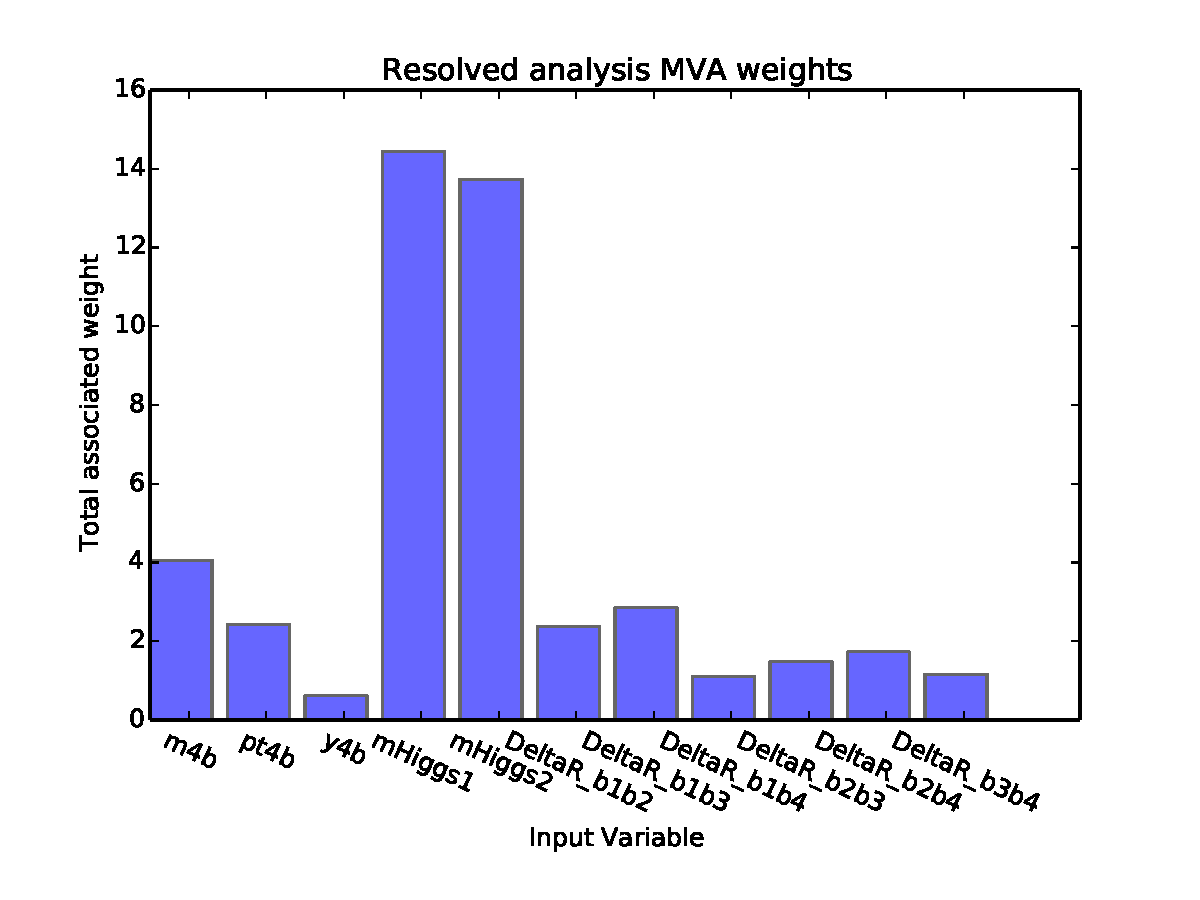
\includegraphics[width=1\textwidth]{plots/nnweights_res.pdf}
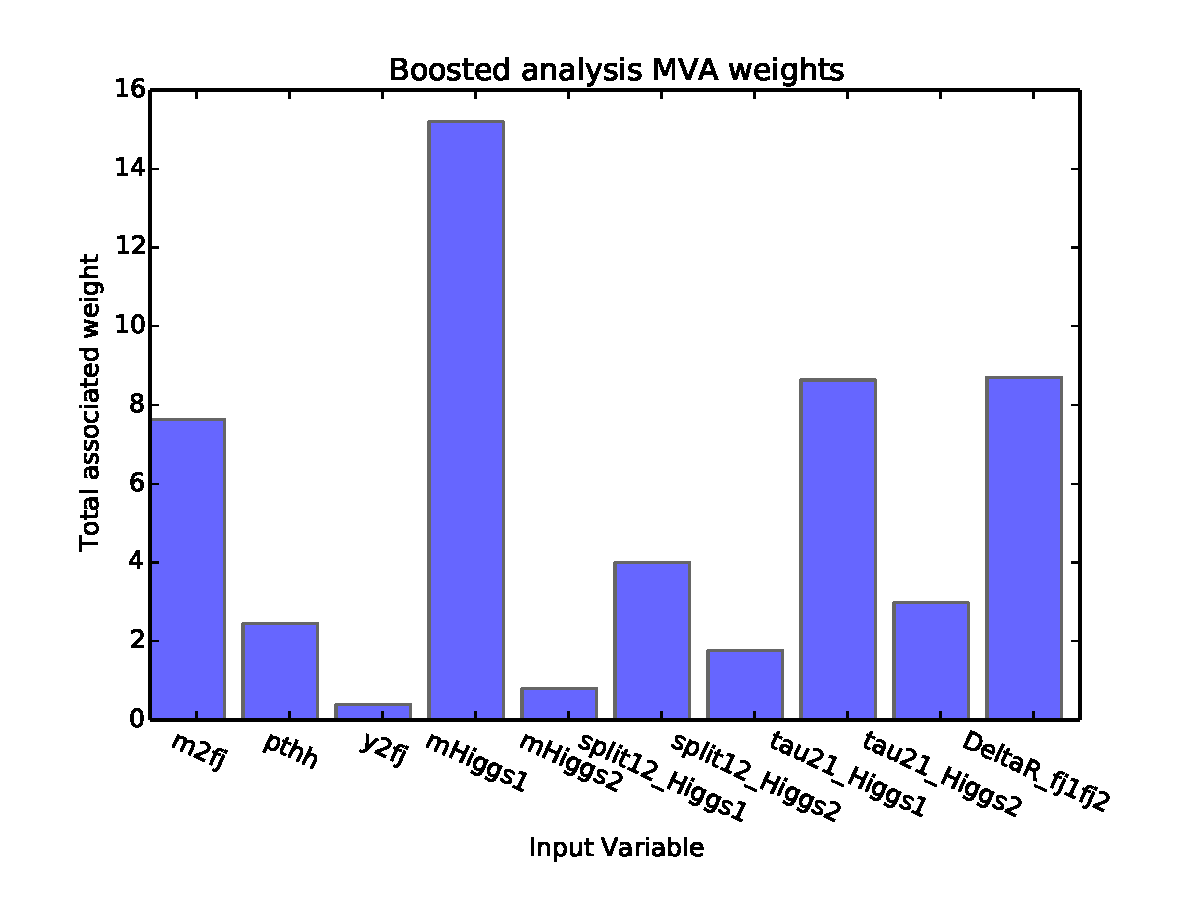
\includegraphics[width=1\textwidth]{plots/nnweights_boost.pdf}
\caption{Distribution of weights per input variable in the final ANN analysis. The above figure shows the weight distribution in the case of the resolved analysis, while the lower plot shows the boosted analysis.}
\label{fig:nnweights}
\end{center}
\end{figure}
\clearpage

Figure~\ref{fig:nnweights} demonstrates that the dijet invariant mass is a crucial variable for the resolved analysis MVA. As no detector effects were modeled in this analysis, it is reasonable to assume that the MVA has greater discriminating power than would be feasible in a real analysis. To investigate this, we now consider a variant of the analysis used in Table~\ref{tab:resCutflow} where the $m_H$ window criterion has been relaxed to $80 < m_H < 170$. Firstly the same analysis is repeated with the larger $m_H$ window. This is then compared to the same analysis but with a Gaussian smearing with $\sigma=10$ GeV applied to the dijet invariant mass used in the MVA. In the left panel of Figure~\ref{fig:invMsmear} the smearing is demonstrated. Despite the smearing, the MVA applied to this analysis still vastly prefers the dijet masses as discriminators, as is demonstrated in the right panel of Figure~\ref{fig:invMsmear}.
  

While the MVA still derives most of it's discriminating power from the dijet masses, the smearing reduces it's effectiveness considerably. In Figure \ref{fig:smearedROC} the ROC curves of the MVA applied to the smeared and unsmeared distributions are shown, where it is clear that the overall performance of the MVA is significantly hampered by the smeared invariant masses. This is echoed in the resulting significance of the analysis as demonstrated in Figure~\ref{fig:smearedSB}
